\begin{frame}{Recursos: Listas}
    \begin{itemize}
    \item Lista simples:
        \begin{itemize}
            \item Item 1
            \item Item 2
        \end{itemize}
    \item Lista Enumerada:
        \begin{enumerate}
            \item Item 1
            \item Item 2
        \end{enumerate}
    \item Lista Personalizada:
        \begin{description}
            \item [<3] Item 1
            \item [<3] Item 2
        \end{description}
    \end{itemize}
\end{frame}
\begin{frame}[fragile]{Código Fonte: Listas}
    \begin{lstlisting}
    Lista simples:
        \begin{itemize}
            \item Item 1
            \item Item 2
        \end{itemize}
    Lista Enumerada:
        \begin{enumerate}
            \item Item 1
            \item Item 2
        \end{enumerate}
    Lista Personalizada:
        \begin{description}
            \item [<3] Item 1
            \item [<3] Item 2
        \end{description}
    \end{lstlisting}
\end{frame}

\begin{frame}{Recursos: Blocos}
    \begin{block}{Esse é um bloco}
        Isso é um teste
    \end{block}
    \begin{block}{}
        Bloco sem título	
    \end{block}
    \begin{alertblock}{Alerta}
        Esse é um alerta
    \end{alertblock}
\end{frame}
\begin{frame}[fragile]{Código Fonte: Blocos}
    \begin{lstlisting}
    $\backslash$begin{frame}{Blocos}
    $\backslash$begin{block}{Esse é um bloco}
    Isso é um teste
    $\backslash$end{block}
    %
    $\backslash$begin{block}{}
    Bloco sem título	
    $\backslash$end{block}
    %
    $\backslash$begin{alertblock}{Alerta}
    Esse é um alerta
    $\backslash$end$\{$alertblock$\}$
    \end{lstlisting}
\end{frame}

\begin{frame}{Recursos: Figura}
    \begin{figure}[h!]
        \centering
        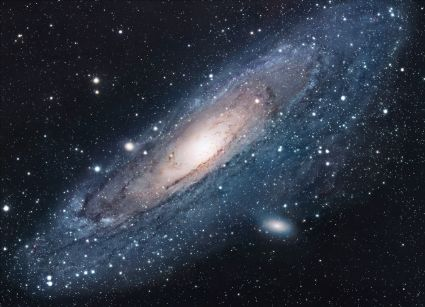
\includegraphics[scale=2]{img/universe.jpg}
        \caption{Isso é uma figura massa!}
        \label{fig:univerise}
    \end{figure}
\end{frame}
\begin{frame}[fragile]{Código Fonte: Figura}
    \begin{lstlisting}
    $\backslash$begin{figure}[h!]
    \centering
    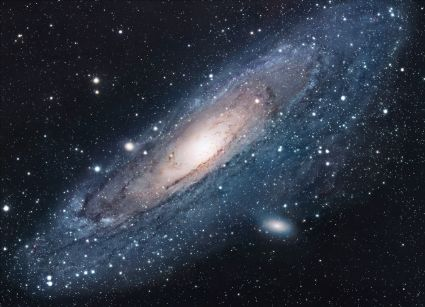
\includegraphics[scale=2]{img/universe.jpg}
    \caption{Isso é uma figura massa!}
    \label{fig:univerise}
    $\backslash$end{figure}
    \end{lstlisting}
\end{frame}

\begin{frame}{Recursos: Tabelas}
    \begin{table}[ht]
        \centering
        \begin{tabular}    {p{0.15\linewidth}p{0.15\linewidth}p{0.15\linewidth}p{0.15\linewidth}p{0.15\linewidth}}
            \hline
            coluna 1 & coluna 2 & coluna 3 & coluna 4 & coluna 5\\
            \hline
            1 & 2 & 3 & 4 & 5\\
            6 & 7 & 8 & 9& 10\\
            11 & 12 & 13 & 14 & 15\\
            16 & 17 & 18 & 19 & 20\\
            21 & 22 & 23 & 24 & 25\\
            \hline
        \end{tabular}
        \caption{Tabela de uma coluna num documento de várias colunas.}
    \end{table}
\end{frame}
\begin{frame}[fragile]{Código Fonte: Tabelas}
    \begin{lstlisting}
    \begin{table}[ht]
        \centering
        \begin{tabular}    {p{0.15\linewidth}p{0.15\linewidth}p{0.15\linewidth}p{0.15\linewidth}p{0.15\linewidth}}
            \hline
            coluna 1 & coluna 2 & coluna 3 & coluna 4 & coluna 5\\
            \hline
            1 & 2 & 3 & 4 & 5\\
            6 & 7 & 8 & 9& 10\\
            11 & 12 & 13 & 14 & 15\\
            16 & 17 & 18 & 19 & 20\\
            21 & 22 & 23 & 24 & 25\\
            \hline
        \end{tabular}
        \caption{Tabela de uma coluna num documento de várias colunas.}
    \end{table}
    \end{lstlisting}
\end{frame}


\begin{frame}{Recursos: Fórmulas}
    \begin{itemize}
            \item A famosa $e=mc^2$ de Albert Einstein !
            \item []
            \item Já essa: \[ e=\lim_{n \to \infty} \left(1+\frac{1}{n}\right)^n \] não é tão famosa assim...
            \item Imaginem essa:
            $$\left|{1\over N}\sum_{n=1}^N \gamma(u_n)-{1\over 2\pi}\int_0^{2\pi}\gamma(t){\rm d}t\right| \le {\varepsilon\over 3}.$$
    \end{itemize}
\end{frame}
\begin{frame}{Código Fonte: Fórmulas}
    \begin{itemize}
        \item Bom, melhor não ver agora...\\Acredite em mim, vai chegar a hora certa!
    \end{itemize}
\end{frame}
\begin{frame}[fragile]{Código Fonte: Fórmulas}
    \begin{itemize}
        \item Ok, vamos ver uma...
        \item []
        \begin{equation}
            \begin{array}{c}
                \underset{x\epsilon S^{n}}{\min}(f_{1}(x),\ldots,f_{k}(x));\quad
                \textrm{sujeito a }
                    \begin{cases}
                        g_{i}(x)\geq0\\
                        g_{l}(x)=0\\
                        x\epsilon S^{n}
                    \end{cases}
            \end{array}
            \label{eqn:1}
        \end{equation}
    \end{itemize}
    \begin{lstlisting}
    \begin{equation}
        \begin{array}{c}
            \underset{x\epsilon S^{n}}{\min}(f_{1}(x),\ldots,f_{k}(x));\quad
            \textrm{sujeito a }
            \begin{cases}
                g_{i}(x)\geq0\\
                g_{l}(x)=0\\
                x\epsilon S^{n}
            \end{cases}
        \end{array}
        \label{eqn:1}
    \end{equation}
    \end{lstlisting}
\end{frame}

\begin{frame}{Don't Panic!}
    \begin{alertblock}{Não entre em Pânico!}
        A maioria dos editores específicos de \LaTeX possuem interfaces gráficas para construções das tabelas, fórmulas, gráficos...\\
    \end{alertblock}
\end{frame}

%parâmetros: linguagem (shell, java, matlab, python, c, php) e arquivo

%\includecode[shell]{codigos/ola.sh}
%
%\includecode[matlab]{codigos/matlab.m}

%ou
% invocar os comandos \ansic, \java, \shell e colocar o código no próprio slide


\begin{frame}[fragile]{Recursos: Códigos}
    
    \includecode[ansic]{codigos/ola.c}	
    
    \ansic
    \begin{lstlisting}
    int main(void){
    printf("Ola mundo\n");
    return 0;
    }
    \end{lstlisting}
    \java
    
    \begin{lstlisting}
    public static voi main(String args[]){
    System.out.println("Ola mundo");
    }
    \end{lstlisting}	
    
\end{frame} 
\begin{frame}[fragile]{Código Fonte: Códigos}
    \begin{lstlisting}
    \begin{lstlisting}
    \includecode[ansic]{codigos/ola.c}	
    
    \ansic
    \begin{lstlisting}
        int main(void){
        printf("Ola mundo\n");
        return 0;
    }
    \ end{lstlisting}
    \end{lstlisting}

    \begin{lstlisting}
    \java
    \begin{lstlisting}
        public static voi main(String args[]){
        System.out.println("Ola mundo");
    }
    \ end{lstlisting}
    \end{lstlisting}
    
\end{frame} 